\documentclass{article}
\usepackage[utf8]{inputenc}
\usepackage{array}
\newcolumntype{C}[1]{>{\centering\arraybackslash}m{#1}}
\usepackage{amsmath}
\usepackage{relsize}
\usepackage{graphicx}

\usepackage[noabbrev]{cleveref}

\crefformat{section}{\S#2#1#3}
\crefformat{subsection}{\S#2#1#3}
\crefformat{subsubsection}{\S#2#1#3}
\crefformat{figure}{#2Figura~#1#3}
\crefformat{footnote}{#2\footnotemark[#1]#3}
\crefformat{table}{#2Tabella~#1#3}
\crefformat{equation}{#2Equazione~#1#3}
\crefformat{chapter}{#2Capitolo~#1#3}

\usepackage{tikz}
\usetikzlibrary{trees}

\begin{document}

\include{title}
\thispagestyle{empty}
\newpage

\section*{Richiami teorici} \label{s:theory}

Nello svolgimento degli esercizi sono stati utilizzati i seguenti concetti teorici.

\paragraph{Notazione $O$}
Data una funzione $g(n)$, $O(g(n))$ indica un insieme di funzioni $f(n)$ in cui:
\begin{itemize}
    \item \begin{equation*}
        O(g(n)) = \{f(n): \exists c > 0: 0 \leq f(n) \leq cg(n), \; \forall n \geq 0\}
    \end{equation*}
    \item $g(n)$ è un limite superiore per $f(n)$;
\end{itemize}

\paragraph{Relazioni di dominanza elementari}
In termini di $O$, vale la seguente catena di disuguaglianze:
\begin{equation}
    1 << log(n) << n << n log(n) << n^2 << n^3 << 2^n << n!
    \label{eq:basic}
\end{equation}

\paragraph{Proprietà di $O$}
In termini di $O$, valgono le seguenti proprietà:
\begin{itemize}
    \item $f(n) + g(n) = O(max(f(n), g(n)))$;
    \item $O(c f(n)) = O(f(n))$;
    \item $O(f(n)) \cdot O(g(n)) = O(f(n) \cdot g(n))$;
\end{itemize}

\paragraph{Sommatorie note}
Negli esercizi, sono state sfruttate le seguenti formule:
\begin{equation}
    \mathlarger{\sum}_{i=m}^{n}(x^i) = \frac{x^{n+1}-x^m}{x-1},con\; x\neq1
    \label{eq:finite_sum}
\end{equation}
\begin{equation}
    \mathlarger{\sum}_{k=1}^{n}(k) = \frac{n(n+1)}{2}
    \label{eq:first_n_sum}
\end{equation}

\paragraph{Teorema dell'esperto}
Data una ricorrenza nella forma $T(n) = aT\left(\frac{n}{b}\right) + f(n))$ e sia $c = \log_b(a)$, il teorema dell'esperto permette di calcolare facilmente un limite alla complessità delle ricorrenze, secondo la tabella sottostante:

\begin{center}
    \begin{tabular}{ | C{5.0cm} | C{5.0cm} |}
        \hline
        Condizione &  Risultato \\ [2ex] 
        \hline\hline
        $f(n) = O(n^c)$ & $T(n) = \Theta(n^c)$ \\  [2ex]
        \hline
        $f(n) = \Theta(n^c\cdot\log^k(n))$ & $T(n) = \Theta(n^c\cdot\log^{k+1}(n))$ \\ [2ex]
        \hline
        $f(n) = \Omega(n^{c+\epsilon}\cdot\log^k(n))$ e $a f(n/b)\leq cf(n)\; con\; c<1$ & $T(n) = \Theta(f(n))$ \\ [2ex]
        \hline
    \end{tabular}
\end{center}
\newpage
\section{Esercizio 1}

Per ogni gruppo di funzioni, ordina le funzioni in ordine crescente di complessità asintotica.

\subsection{Blocco 1}

\begin{equation*}
    \begin{split}
        & f_1(n) = n^{0.99999} log(n) \\
        & f_2(n) = 1000000\; n \\
        & f_3(n) = 1.000001^n\\
        & f_4(n) = n^2
    \end{split}
\end{equation*}

La soluzione è:
\begin{equation*}
    f_1(n) < f_2(n) < f_4(n) < f_3(n) 
\end{equation*}
In cui, per la funzione $log(n)$, si è sfruttata la proprietà $O(n^{0.99999}\cdot n^{0.00001}) = O(n)$, mentre per le altre si è utilizzata l'\cref{eq:basic}.

\subsection{Blocco 2}

\begin{equation*}
    \begin{split}
        & f_1(n) = 2^{2^{1000000}}\\
        & f_2(n) = 2^1000000\; n \\
        & f_3(n) =  \binom{n}{2} \\
        & f_4(n) = n\sqrt{n}
    \end{split}
\end{equation*}

La soluzione è:
\begin{equation*}
    f_1(n) < f_4(n) < f_3(n) < f_2(n) 
\end{equation*}
In cui, $f_1(n)$ ha una complessità costante; mentre applicando la definizione di coefficiente binomiale a $f_3(n)$ ottiene che:
\begin{equation*}
    \binom{n}{2} = \frac{n!}{2! \; (n - 2)!} = \frac{n\; (n-1)}{2!} = O(n^2)
\end{equation*}
Infine, applicando la \cref{eq:basic} si arriva al risultato ordinando $f_4(n) < f_3(n)$ e ponendo $f_2(n)$ alla fine della catena di disuguaglianze.

\subsection{Blocco 3}

\begin{equation*}
    \begin{split}
        & f_1(n) = n^{\sqrt{n}} \\
        & f_2(n) = 2^n \\
        & f_3(n) = n^{10}\; 2^{\frac{n}{2}} \\
        & f_4(n) =  \sum_{i=0}^{n}(i+1) \\
    \end{split}
\end{equation*}

La soluzione è:
\begin{equation*}
    f_4(n) < f_1(n) < f_3(n) < f_2(n) 
\end{equation*}
In cui, $f_1(n) = O(2^{log(n)\sqrt{n}})$ e $f_3(n) = O(2^{10log(n) + n})$ confrontando il comportamento asintotico si ottiene che $f_2(n) < f_3(n)$. Mentre, applicando la linearità e la formula per la somma corrente dei primi $n$ numeri naturali a $f_4(n)$ si ottiene che:
\begin{equation*}
    \sum_{i=0}^{n}(i+1) = \sum_{i=0}^{n}(i) + \sum_{i=0}^{n}(1) = \frac{n\; (n+1)}{2} + n -1  = O(n^2)
\end{equation*}
Infine, applicando la \cref{eq:basic} si arriva al risultato ordinando $f_4(n) < f_1(n)$ e confrontando gli esponenti delle funzioni esponenziali di base $2$.

\section{Esercizio 2}

Per ognuna delle seguenti funzioni si determini se $f(n) = O(g(n)), g(n) = O(f(n))$ o entrambe.

\begin{center}
    \begin{tabular}{ | C{2.8cm} | C{2.8cm} | C{2.4cm} | C{2.4cm} |}
        \hline
        $f(n)$ & $g(n)$ & $f(n) = O(g(n))$ &  $g(n) = O(f(n))$ \\ [2ex] 
        \hline\hline
        $\frac{n^2-n}{2}$ & $6n$ &  & X \\  [2ex] 
        \hline
        $n+2\sqrt{n}$ & $n^2$ & X &  \\  [2ex] 
        \hline
        $n\;log(n)$ & $n\sqrt{\frac{n}{2}}$ & X &  \\  [2ex] 
        \hline
        $n + log(n)$ & $\sqrt{n} $ &  & X \\  [2ex] 
        \hline
        $2\;log^2(n)$ & $log(n) + 1 $ &  & X \\  [2ex] 
        \hline
        $4n\;log(n)+n$ & $\frac{n^2-n}{2}$ & X &  \\ [2ex] 
        \hline
    \end{tabular}
\end{center}

Per ogni coppia di funzioni, si è applicata la \cref{eq:basic}, avvalendosi delle proprietà di $O$ indicate in precedenza.

\section{Esercizio 3}
Si indichi se le seguenti affermazioni sono vere o false.

\paragraph{1. $2^{(n+1)} = O(2^n)$} L'affermazione è vera. Utilizzando le proprietà delle potenze è possibile scrivere $2^{n+1} = 2\cdot2^n$ e quindi sapendo che $O(c f(n)) = O(f(n))$, la proprietà risulta vera $\forall c\geq2$.

\paragraph{2. $2^{2n} = O(2^n)$} L'affermazione è falsa. Mediante le proprietà delle è potenze, è possibile scrivere il primo membro della relazione come $2^{n^2}$, mentre esplicitando il termine $O(2^n)$ con $c2^n$, possiamo effettuare il confronto e ottenere $2^{2^n} \leq c2^n$. Applicando le proprietà dei logaritmi, si trova che $2n log(2) \leq log(c) + n log(2)$ e, semplificando, si trova che $n \leq log(c)$, ma la relazione ottenuta non è mai vera per nessun valore di $c$.

\section{Esercizio 4}
Fornire il limite inferiore e superiore per T(n) nelle seguenti ricorrenze, usando il metodo dell’albero delle ricorrenze ed il teorema dell’esperto se applicabile. Si fornisca il limite più stretto possibile giustificando la risposta.

\subsection{Riccorrenza 1}
\begin{equation*}
   T(n) = 2T\left(\frac{n}{2}\right) + O(\sqrt{n})
\end{equation*}

\subsubsection{Albero delle ricorrenze}
Nello schema sottostante, è mostrato l'albero di ricorrenze, partendo dalla $f(n) = c\cdot\sqrt{n}$. Sviluppando ricorsivamente la relazione iniziale si arriva al caso generale $T\left(\frac{n}{2^i}\right)$ con cui è possibile ricavare il caso elementare $T(1)$. Applicando $1 = \left(\frac{n}{2^i}\right)$ si ottiene che $i = \log_2(n)$. Il costo di ogni livello è $c\cdot\sqrt{2^i\cdot n}$. Quindi, per trovare il costo totale, bisogna sommare il costo per livello fino ad arrivare al caso base, ottenendo $\mathlarger{\sum}_{i=0}^{\log_2(n)} (c\sqrt{2^i\cdot n})$ che può essere risolta applicando l' \cref{eq:finite_sum} e sfruttando che $a = b^{\log_b(a)}$ ottenendo $c\sqrt{n}\cdot \frac{\sqrt{n}-1}{\sqrt{2}-1}$. Essendo il denominatore costante, risulta trascurabile nella notazione $O$ e, quindi, svolgendo i prodotti al numeratore risulta $c\cdot\frac{n-\sqrt{n}}{\sqrt{2}-1}$ che può essere maggiorata da $O(n)$. 


\begin{tikzpicture}[level 1/.style={sibling distance=5.6cm},level 2/.style={sibling distance=3cm},level 3/.style={sibling distance=2cm}]
	\node {$c\sqrt{n}$}[edge from parent fork down]
        
		child { node {$c\sqrt{n/2}$}
			child { node {$c\sqrt{n/4}$} 
			    child {node{$c\sqrt{n/8}$}}
			    child {node{...}}
			    }
			child { node {$c\sqrt{n/4}$} 
			    child {node{...}}
			    child {node{...}}
			    }
			}	
		child { node {$c\sqrt{n/2}$}
			child { node {$c\sqrt{n/4}$} 
			    child {node{...}}
			    child {node{...}}
			    }
			child { node {$c\sqrt{n/4}$} 
			    child {node{...}}
			    child {node{...}}
			    }
			}	
	;
\end{tikzpicture}

\subsubsection{Metodo dell'esperto}
In questo caso, il metodo dell'esperto si applica immediatamente in quanto la ricorrenza è già nella forma nota. Essendo $a=2\;e\;b=2$, si ottiene che $c=\log_2(2) = 1$, mentre $f(n) = \sqrt{n}$. Quindi dato che, $n^{\frac{1}{2}} = O(n)$, si ricade nel primo caso del teorema dell'esperto e, pertanto, $T(n) = \Theta(n)$.


\subsection{Ricorrenza 2}

\begin{equation*}
   T(n) = T\left(\sqrt{n}\right) + \Theta(\log\log(n))
\end{equation*}

\subsubsection{Albero delle ricorrrenze}
Per ricondurre, l'esercizio alla forma nota del tipo $T(n) = aT\left(\frac{n}{b}\right)$ si è scelto di adoperare la sostituzione  $n = 2^k$. Svolgendo i calcoli, si ottiene $T(2^k) = T\left(2^{\frac{k}{2}}\right) + c\cdot\log\log2^k$. Considerando $y(k) = T(2^k)$, si ottiene la ricorrenza $y(k) = y\left(\frac{k}{2}\right) + c\cdot\log(k)$ usando la relazione $\log_a(b)^k = k \cdot \log_a(b)$. Nello schema sottostante, è stato sviluppato l'albero delle ricorrenze relativo a $y(k)$. Come nell'esercizio precedente, il caso $y(1)$ è dato da $1 = \frac{k}{2^i}\Rightarrow i=\log_2(k)$. Dalla struttura dell'albero si ricava che il costo totale è dato quindi da $\mathlarger{\sum_{i=0}^{\log_2(k)}}(c\cdot\log(\frac{k}{2^i}))$ che, usando le proprietà di somma dei logaritmi, viene divisa in
\begin{equation*}
    c\cdot\left(\mathlarger{\sum}_{i=0}^{\log_2(k)}(\log(k)) +\mathlarger{\sum}_{i=0}^{\log_2(k)}(\log\left(\frac{1}{2^i}\right))\right)
\end{equation*}


Nella prima sommatoria, il logaritmo non dipende a $i$, quindi il risultato è semplicemente $\log_2(n)$; mentre la seconda, sfruttando le proprietà di somma dei logaritmi, equivale a $\log(\mathlarger{\prod}_{i=0}^{\log_2(k)}(\frac{1}{2^i}))$ che è sicuramente trascurabile rispetto al prodotto di due funzioni logaritmiche. Quindi si ottiene $y(k) = O(log^2(k))$. Tornando alla sostituzione iniziale, si ottiene che $n = 2^k \Rightarrow k = \log(n)$ e, sostituendo nel risultato precedente si ottiene che $T(n) = O(\log^2\log(n))$.

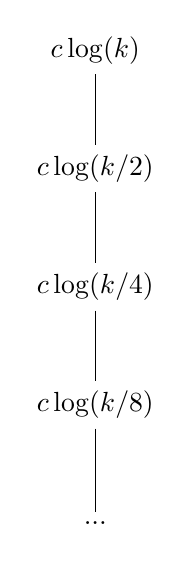
\begin{tikzpicture}[level 1/.style={sibling distance=1.15cm},level 2/.style={sibling distance=3cm},level 3/.style={sibling distance=2cm}]
	\node {$c\log(k)$}[edge from parent fork down]
		child { node {$c\log(k/2)$}
		    child {node{$c\log(k/4)$}
		        child {node{$c\log(k/8)$}
		             child {node{...}}
		            }
		    }
		}
	;
\end{tikzpicture}

\subsubsection{Teorema dell'esperto}
Analogamente a come fatto nell'albero delle ricorrenze, per ricondurci alla forma nota che consente di applicare il teorema dell'esperto si effettua la sostituzione $n = 2^k$. Quindi, ottenuta la sommatoria di appoggio $y(k) = y\left(\frac{k}{2}\right) + c\cdot\log(k)$, si ricade nel caso 3 del teorema dell'esperto con $c=\log_2(1) = 0$ e, pertanto, risulta $y(k) =  \Theta(\log(k))$. Quindi, tornando alla sostituzione $2^k=n$, si ottiene che $T(n) = O(\log^2\log(n))$.

\subsection{Ricorrenza 3}

\begin{equation*}
   T(n) = 10T\left(\frac{n}{3}\right) + 17(n)^{1.2}
\end{equation*}

\subsubsection{Albero delle ricorrenze}

Nello schema sottostante, è mostrato l'albero di ricorrenze (semplificato per favorirne la lettura), partendo dalla $f(n) = 17(n/3)^{1.2}$.
Come negli esercizi precedenti è stata sviluppata la ricorsione, in cui ogni nodo ha 10 figli, arrivando alla relazione generale $17(n/3^i)^{1.2}$ e calcolando $i = \log_3(n)$.
La somma totale dei costi può essere calcolata come $\mathlarger{\sum}_{i=0}^{\log_3(n)} (17\cdot 10^i(\frac{n}{3^i})^{1,2})$ che, portando fuori i termini non dipendenti dalla i, e applicando la somma descritta nella \cref{eq:finite_sum}, diventa:
\begin{equation*}
    17n^{1.2} \cdot \mathlarger{\sum}_{i=0}^{\log_3(n)} (2,67^i) \leq 10 \cdot n^{1.2} (n-1) = O(n^{2.2})
\end{equation*}

\begin{tikzpicture}[level 1/.style={sibling distance=1.15cm},level 2/.style={sibling distance=3cm},level 3/.style={sibling distance=2cm}]
	\node {$17n^{1.2}$}[edge from parent fork down]
		child { node {$17(n/3)^{1.2}$}
		    child {node{$17(n/9)^{1.2}$  ...}
		        child {node{$17(n/27)^{1.2}$  ...}
		            child { node {...}}	
		            }
		    }
		}
		child { node {...}}
		child { node {...}}
		child { node {...}}
		child { node {...}}
		child { node {...}}
		child { node {...}}
		child { node {...}}
		child { node {...}}
		child { node {...}}
	;
\end{tikzpicture}

\subsubsection{Metodo dell'esperto}
In questo caso, il metodo dell'esperto si applica immediatamente in quanto la ricorrenza è già nella forma nota. Essendo $a=10\;e\;b=3$, si ottiene che $c=\log_3(10) \approx 2.1$, mentre $f(n) = 17n^{1.2}$. Quindi dato che, $n^{1.2} = O(n^{2.1})$, si ricade nel primo caso del teorema dell'esperto e, pertanto, $T(n) = \Theta(n^{2.1})$.

\subsection{Ricorrenza 4}
Dimostrare che:
\begin{equation*}
    T(n) = T\left(\frac{n}{3}\right) + T\left(\frac{2n}{3}\right) + cn = \Omega(n\cdot \log(n)), con\;c\;costante
\end{equation*}

Innanzitutto è stato sviluppato l'albero delle ricorrenze in cui ogni nodo si dirama in due figli: nel sinistro si richiama $T\left(\frac{n}{3}\right)$; mentre nel destro $T\left(\frac{2n}{3}\right)$. Il costo totale per ogni livello è sempre $c\cdot n$. Volendo calcolare il limite asintotico inferiore, $\Omega(\cdot)$, bisogna considerare il caso migliore, cioè il percorso più breve. In questo caso, è possibile notare che il percorso più veloce è ottenuto seguendo il ramo di sinistra generato dalla chiamata ricorsiva $T\left(\frac{n}{3}\right)$: $n,cn\left(\frac{1}{3}\right), cn\left(\frac{1}{3}\right)^2 ,\dots, 1 $. La lunghezza del percorso di sinistra è $\log_3(n)$. Quindi il costo totale è dato da $\log_3(n)\cdot cn = \Omega(n\cdot\log(n))$.

\begin{tikzpicture}[level 1/.style={sibling distance=5.6cm},level 2/.style={sibling distance=3cm},level 3/.style={sibling distance=2cm}]
	\node {$cn$}[edge from parent fork down]
		child { node {$c(n/3)$}
			child { node {$c(n/9)$}
			    child {node{...}}
			    child {node{...}}
			    }
			child { node {$c(2n/9)$}
			    child {node{...}}
			    child {node{...}}
			    }
			}
		child { node {$c(2n/3)$}
			child { node {$c(2n/9)$}
			    child {node{...}}
			    child {node{...}}
			    }
			child { node {$c(4n/9)$}
			    child {node{...}}
			    child {node{...}}
			    }
			}
	;
\end{tikzpicture}


\section{Problemi}

\subsection{Problema 1}

La soluzione prevede l'utilizzo di una doppia \textit{linked list} in cui, per ogni nodo, si hanno sia il puntatore a quello precedente che a quello successivo e viene tenuto traccia del numero di elementi presenti nella struttura attraverso la variabile $n$. La funzione \textit{half\_reverse} inverte gli elementi della lista ignorando i primi $\frac{n}{2}$.
Alla riga 17, vengono inizializzati i puntatori di appoggio:
\begin{itemize}
    \item \textit{current}: viene utilizzato per scorrere la lista in avanti;
    \item \textit{prev} e \textit{next}: tengono traccia degli elementi precedenti e successivi di \textit{current} per la procedura di \textit{swap};
    \item \textit{last}: serve a tenere traccia dell'elemento precedente a quello da cui parte la procedura di inversione della lista;
\end{itemize}

Una volta saltati i primi $\frac{n}{2}$ elementi con il ciclo \textit{for} alla riga 18, viene salvato l'elemento precedente al \textit{current} in \textit{last}. Nelle righe 23-27, viene svolta la procedura \textit{swap} invertendo la posizione dell'elemento corrente con il successivo fino a quando non si arriva alla fine della lista. Infine, alla riga 29, viene utilizzato il puntatore \textit{last} per ricongiungere la metà invertita con la prima.

\paragraph{Complessità}
La complessità della funzione half\_reverse è $O(n)$ poiché vengono eseguiti due cicli, non innestati, che effettuano ciascuno al più $\frac{n}{2}$ iterazioni.


\subsection{Problema 2}
Il problema può essere diviso in due sotto-problemi: trovare il numero degli elementi minori dell'i-esimo all'interno di un vettore e scrivere il risultato in un secondo vettore nell' i-esima posizione (in $O(n\log(n))$). Inoltre, va gestita la possibilità che esistano elementi duplicati. Lo schema di funzionamento della soluzione è mostrato in \cref{fig:find_min}.

\paragraph{Ricerca degli elementi minori}
Questo problema è stato partendo da una versione ordinata del vettore di partenza. In questo modo, scorrendo il vettore in maniera crescente, per ogni elemento il numero di minori è pari alla sua posizione. Se ci sono duplicati, il risultato descritto in precedenza, relativo al primo elemento trovato, deve essere incrementato del numero di doppioni.

\paragraph{Scrittura dei risultati}
Per scrivere i risultati nella stessa posizione originale rispettando il vincolo della complessità $O(n\log(n))$ si è scelto di introdurre una struttura dati ausiliaria. In particolare, è stato creato un dizionario (implementato nella \textit{stl} attraverso una \textit{hash table} nella classe \textit{std::unordered\_map}) le cui chiavi corrispondono ai possibili elementi del vettore a cui sono associati dei vettori contenenti le posizioni nell'\textit{array} di partenza. In questo modo, è possibile calcolare il risultato come $i+positions.size() -1$ dove \textit{positions} è il vettore delle posizioni conservato nella mappa.

\begin{figure}[htp]
    \includegraphics[width=12cm]{pog.png}
    \centering
    \caption{Procedura find\_min}
    \label{fig:find_min}
\end{figure}

\paragraph{Complessità}
La complessità della funzione find\_min è $O(n+n\log(n)+n)=O(n\log(n))$. Il primo ciclo scorre tutti gli elementi del vettore e popola la mappa (\textit{std::unordered\_map} fornisce operazioni con complessità costanti al netto della procedura di \textit{hash}). La funzione di ordinamento utilizzata è \textit{std::stable\_sort}, che garantisce una complessità massima di $n\log(n)$. Infine vengono eseguiti due cicli innestati che però in totale effettuano al massimo $n$ iterazioni.


\subsection{Problema 3}
Per implementare la struttura \textit{treap} ogni nodo è stato dotato di una variabile \textit{priority} il cui valore viene generato casualmente al momento della creazione di un nuovo nodo.
La procedura di \textit{treap\_insert} è basata sull'inserimento in un BST. Dopo, il classico inserimento nell'albero (in cui ogni figlio sinistro è minore del padre, mentre quello destro è maggiore) viene effettuato un controllo sulla priority tramite la funzione ricorsiva \textit{min\_heapify} che si occupa di mantenere la proprietà secondo cui i figli hanno maggiore priorità del padre. Per farlo, sono state implementate due funzioni di rotazione (\textit{left\_rotate} e \textit{right\_rotate}). \textit{right\_rotate} viene chiamata se il nodo in cui la proprietà viene violata è il figlio di sinistra, \textit{left\_rotate} altrimenti.

Per eseguire una rotazione, ad esempio quella a destra (\cref{fig:right_rotation}), vengono svolti i seguenti passaggi:
\begin{figure}[htp]
    \includegraphics[width=11cm]{rotation2.png}
    \centering
    \caption{Procedura di \textit{right rotation}}
    \label{fig:right_rotation}
\end{figure}

\paragraph{Complessità}
La complessità della procedura \textit{treap\_insert} differisce da quella del BST a causa delle rotazioni necessarie. Al primo inserimento, il numero di rotazioni necessarie è zero, al secondo massimo una, al terzo al più $\log_2 (3)$ e generalizzando si effettuano $O(h)$ rotazioni. Essendo la complessità dell'inserimento del BST $O(h),\;con\; h=O(\log(n))$, quella totale sarà $O(2h) = O(\log(n))$

\end{document}
